% What Holds Up in a Second Period? -- conference draft (ACM sigconf, ICAIF format).
% Build: latexmk -pdf main.tex
% Numbers come from runs/paper/week/signals.csv and results.csv (6 decimals, rounded half-up).
\documentclass[sigconf,nonacm]{acmart}

\usepackage{booktabs}
\usepackage{tabularx}
\usepackage{array}
\usepackage{multirow}
\usepackage{pgfplots}
\usepgfplotslibrary{groupplots}
\pgfplotsset{compat=1.18}
\usetikzlibrary{positioning,arrows.meta}

\definecolor{TestBlue}{HTML}{2A78D6}
\definecolor{ValOrange}{HTML}{EB6834}
\definecolor{Teacher}{HTML}{14365E}
\definecolor{Muted}{HTML}{666666}
\definecolor{Rule}{HTML}{BBBBBB}

\newcommand{\rng}[2]{{\scriptsize[#1, #2]}}
\newcommand{\hold}{\textbf{Holds}}

\settopmatter{printacmref=false}
\renewcommand\footnotetextcopyrightpermission[1]{}

\begin{document}

\title{What Holds Up in a Second Period?}
\subtitle{Distilling Earnings-Call Reading from a Frontier LLM into a Laptop Model}

\author{Nityanand Rai}
\orcid{0009-0002-2196-5023}
\affiliation{%
  \institution{Independent researcher}
  \country{USA}}

\begin{abstract}
We test whether a small open-weight language model can learn to read earnings calls from a frontier model and then rank stocks.
We call the small model the student and the frontier model the teacher.
The student is Qwen3.5-9B, quantized to 4 bits, on one laptop with 18\,GB of memory.
The teacher is Claude Opus 5.5.
We compare six setups on one ladder, where each step adds one thing.
The setups are facts only, call text, retrieval, agentic search, fine-tuning on teacher labels, and reinforcement learning (RL) with a trade reward.
Each setup writes a short read of the business and an action, BUY or AVOID.
We score 800 small-cap calls from March to August 2026, after the student's release.
Then we repeat every check on 500 calls from 2025.
We measure skill with information coefficients (ICs), the correlation of a setup's scores and the real outcomes, ranked within each month.
The Stock IC uses the stock's return against its sector over the next 60 trading sessions.
The EPS IC uses the next change in earnings per share (EPS).
Three results hold.
First, every setup forecasts the direction of the next EPS change, with an EPS IC of 0.16 to 0.28 in both periods.
But a one-line rule on the last EPS change does almost as well.
Second, the model's action follows its own read of the call.
Third, the teacher ranks stocks better than the trained student on all 2026 calls.
After the teacher's knowledge date, the end of its training data, the gap is not distinguishable from zero.
Most other gains do not repeat.
Stock ICs of about 0.10 in 2026 fall to about zero in 2025.
The return after costs of the RL model changes from $+1.06\%$ to $-2.08\%$.
Controls trained on shuffled labels match the trained models.
A single test period would have overstated the skill of every setup.
We release the code, the trained adapters and all scores.
\end{abstract}

\keywords{earnings calls, knowledge distillation, reinforcement learning, small language models, evaluation, look-ahead bias}

\maketitle

%======================================================================
\section{Introduction}
%======================================================================

Large language models (LLMs) read financial text well, and their reads of news can predict returns~\cite{lopezliratang2023}.
Frontier models are expensive to run on thousands of documents.
Small open models are free to run on a laptop, but they read less well.
Distillation~\cite{hinton2015} is the usual bridge: train the small model on the large model's answers.
We call the small model the \emph{student} and the large model the \emph{teacher}.

Two problems make results in this area hard to trust.
First, a model can remember what happened after a document from its pretraining data~\cite{glassermanlin2023,lopezlira2025memorization}.
A model's \emph{knowledge date} is the last date of its training data.
Second, many studies report one test period.
In finance, predictors often weaken outside the sample in which they were found~\cite{mcleanpontiff2016}.
Re-tests of LLM trading strategies over long periods, or after the models' knowledge dates, show the same decay~\cite{li2025finsaber,li2025profitmirage}.
The authors of one LLM finance paper withdrew it after a co-author found inconsistencies in its data and analyses~\cite{kim2024fsa}.

We study one narrow task with both problems in view.
A model reads management's replies to analysts' questions in the earnings call of a small company.
It writes a structured read of the business, a forecast of the next EPS change, and an action, BUY or AVOID.
The action is for a trade that buys at the next open and sells at the close 60 trading sessions (trading days) after the decision.
An \emph{EPS change} is a quarter's earnings per share (EPS) minus the EPS of the same quarter one year earlier.
The \emph{next EPS change} is the change for the quarter after the call.
We test the student on calls after its release date.
Then we repeat every check in a second period.

Our contributions are:
\begin{itemize}
\item \textbf{A controlled ladder.} Six setups share one task, one prompt and one library of documents. Simple rules and two controls trained on shuffled labels sit beside them (Section~\ref{sec:setup}).
\item \textbf{A second-period check of every signal.} A \emph{signal} is a result that suggests skill, such as a gain of one setup over another. We report each signal in 2026 and in 2025, with 95\% bootstrap ranges. Most signals do not repeat (Section~\ref{sec:signals}).
\item \textbf{A teacher comparison on the same calls.} We split the test at the teacher's knowledge date. Memory cannot explain the comparison on the calls after that date (Section~\ref{sec:teacher}).
\item \textbf{An open pipeline on one laptop.} We release the code, the trained adapters and all scores. A sealed test set from the same months stays closed for a confirmatory test (Section~\ref{sec:future}).
\end{itemize}

%======================================================================
\section{Related work}
%======================================================================

\textbf{Text and returns.}
Quarterly EPS changes are autocorrelated, and prices drift after earnings surprises, which are earnings that differ from the forecast~\cite{bernardthomas1990}.
Finance-specific word lists measure the tone of corporate text~\cite{loughranmcdonald2011}.
The tone of call text predicts returns over the 60 trading days after the call~\cite{price2012}.
LLM reads of news headlines predict returns~\cite{lopezliratang2023}.
We use the last EPS change and a word list as baselines, so that a model gain must exceed both.

\textbf{LLM trading agents.}
Agent systems combine memory, tools and several roles, and many use a frontier model at inference time.
Many report one short test window.
For example, TradingAgents reports a three-month backtest~\cite{xiao2024tradingagents}.
StockBench uses a four-month window with no trading costs~\cite{chen2025stockbench}.
FINSABER re-tests LLM strategies over two decades and more than 100 stocks, and the reported advantages fall a lot~\cite{li2025finsaber}.
Tests after the model's knowledge date find similar decay~\cite{li2025profitmirage}.

\textbf{Distillation to small models.}
Trading-R1 distils reasoning traces from large models into a model with 4 billion parameters, then applies reinforcement learning (RL)~\cite{xiao2025tradingr1}.
Earlier work distilled ChatGPT labels of call text into small classifiers~\cite{gandouet2024distilled}.
To our knowledge, neither study compares the student with its teacher after the student's knowledge date, or repeats the test in a second period.
Our study is smaller, but it tests every step of one pipeline in two periods.

\textbf{Look-ahead bias.}
\emph{Look-ahead bias} occurs when a model trained on text from after a document's date knows the outcome of that document.
One way to measure this bias is to hide the company names~\cite{glassermanlin2023}.
But models recall exact values from before their knowledge date, and masking does not stop them from rebuilding names and dates~\cite{lopezlira2025memorization}.
Optimizing a model with supervised fine-tuning (SFT) or RL can recover look-ahead information~\cite{koijenlevy2026}.
We mask names, tickers and years.
We also test only on calls after the student's release, and we split the teacher's test at its knowledge date.

\textbf{Post-training.}
We fine-tune with LoRA~\cite{hu2022lora}, which trains small low-rank adapter matrices while the base model stays frozen.
As in distillation~\cite{hinton2015}, the action target is soft: a probability, not a single label.
In RL, the \emph{policy} is the model's probability of each answer.
Common RL methods for LLMs sample answers and follow the policy gradient.
A Kullback--Leibler (KL) penalty keeps the policy near its start.
With this penalty, the best policy has a closed form: the start policy tilted by the exponential of the reward~\cite{korbak2022kl}.
Our RL step moves the policy toward this target by cross-entropy.

\begin{figure*}[t]
\centering
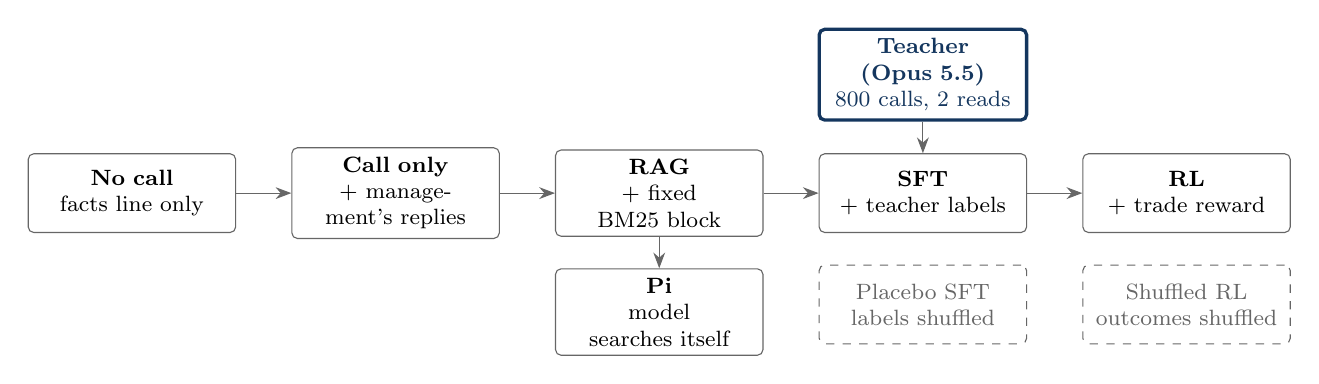
\begin{tikzpicture}[
  node distance=4mm and 7mm,
  box/.style={draw=Muted, rounded corners=2pt, align=center, font=\footnotesize, minimum height=10mm, text width=24mm, fill=white},
  ctl/.style={box, dashed, text=Muted},
  tea/.style={box, draw=Teacher, text=Teacher, very thick},
  arr/.style={-{Stealth[length=2mm]}, draw=Muted}]
\node[box] (nocall) {\textbf{No call}\\facts line only};
\node[box, right=of nocall] (call) {\textbf{Call only}\\+ management's replies};
\node[box, right=of call] (rag) {\textbf{RAG}\\+ fixed BM25 block};
\node[box, right=of rag] (sft) {\textbf{SFT}\\+ teacher labels};
\node[box, right=of sft] (rl) {\textbf{RL}\\+ trade reward};
\node[box, below=of rag] (pi) {\textbf{Pi}\\model searches itself};
\node[ctl, below=of sft] (placebo) {Placebo SFT\\labels shuffled};
\node[ctl, below=of rl] (shuf) {Shuffled RL\\outcomes shuffled};
\node[tea, above=of sft] (teacher) {\textbf{Teacher (Opus 5.5)}\\800 calls, 2 reads};
\draw[arr] (nocall) -- (call);
\draw[arr] (call) -- (rag);
\draw[arr] (rag) -- (sft);
\draw[arr] (sft) -- (rl);
\draw[arr] (rag) -- (pi);
\draw[arr] (teacher) -- (sft);
\end{tikzpicture}
\caption{The ladder. Every setup gets the same facts line and prompt layout. Each arrow changes one thing. Dashed boxes are controls that we broke on purpose.}
\label{fig:ladder}
\end{figure*}

%======================================================================
\section{Setup}\label{sec:setup}
%======================================================================

\subsection{Data}

\textbf{Calls.} We use earnings-call transcripts from a public dataset.\footnote{\url{https://huggingface.co/datasets/defeatbeta/yahoo-finance-data}}
We keep calls of US companies with a share price of \$3 or more.
The median daily dollar volume (price times shares traded) over the 60 sessions before the call must be \$1M to \$50M.
We call these companies \emph{small-cap}, although the filter uses trading volume and not market value.
In the question-and-answer part of the call, management's replies must have at least 300 words, and the analysts' questions at least 100 words.
We draw every call set from the calls that pass this filter.
A script masks the company name, the ticker and the years before any model reads a call.

\textbf{Sets.} A script assigned every call to one set before any model ran, and recorded checksums (Table~\ref{tab:sets}).
The student, Qwen3.5-9B~\cite{qwen2026qwen35}, was released in February 2026.
The teacher is Claude Opus 5.5 (\texttt{claude-opus-5-5}), called through the Anthropic batch API.
Thus it cannot know the outcomes of the test calls.
The SFT and RL sets train the models.
On the check set, we compare the student's read lines with the teacher's.
The validation set is the second period.
A further sealed test set from the same months stays closed for a confirmatory test (Section~\ref{sec:future}).
Only the final scoring script opened the test outcomes.

\begin{table}[t]
\caption{Call sets used in this study.}
\label{tab:sets}
\small
\begin{tabular}{lrl}
\toprule
Set & Calls & Dates \\
\midrule
SFT training & 800 & 2021--2024 \\
RL training & 400 & 2021--2024 \\
Check (teacher comparison) & 300 & 2023--2024 \\
Validation (second period) & 500 & 2025 \\
\textbf{Test} & \textbf{800} & \textbf{Mar--Aug 2026} \\
\bottomrule
\end{tabular}
\end{table}

\textbf{Outcome.} The model decides at the close of the first session after the call.
The trade buys at the next open and sells at the close 60 sessions after the decision.
The excess return is the stock's return minus the mean return of its sector.
The outcome divides the excess return by the usual 60-session move:
\begin{equation}
y = \frac{r_{\text{stock}} - r_{\text{sector}}}{\sigma_{\text{daily}}\sqrt{60}} .\label{eq:y}
\end{equation}
Here $r_{\text{stock}}$ and $r_{\text{sector}}$ are the returns over the trade.
$\sigma_{\text{daily}}$ is the standard deviation of the stock's daily returns over the 60 sessions before the decision.

\textbf{Library.} The \emph{library} is a SQLite file of documents that a model can search.
It holds 604{,}728 passages of management's replies, 56{,}013 outcome cards, quarterly figures of 3{,}103 companies, and 50 analyst notes.
An \emph{outcome card} tells how a past call turned out: whether the stock beat its sector, and whether the next EPS change was up.
The teacher wrote the analyst notes, which give general advice on how to read a call, with no company, date or figure.
Each item has the date from which a search can return it.
An outcome card becomes available only when its 60-session trade closes.
A search never returns the call that the model reads.
Search uses the SQLite full-text index with BM25, a standard keyword-match score, and no embeddings.

\subsection{Task and scoring}

The prompt has four parts: a facts line, an optional \emph{knowledge block} of library documents, management's masked replies, and an instruction.
The knowledge block has up to 1{,}500 tokens, and the replies have up to 2{,}500 words.
The facts line gives the dollar volume, the past 60-session return, the daily volatility, the price move around the call, and the last EPS change.
The model completes seven lines.
The five \emph{read lines} are Demand, Pricing, Margins, Guidance and Candor.
Demand, Pricing and Margins take up, flat or down, over the next two quarters.
Guidance takes raised, held, cut or none, and Candor takes direct or evasive.
Then come Next EPS (up or down) and Action (BUY or AVOID).

We do not sample free text.
At each line, a script reads the probabilities of the allowed values and normalizes them to a sum of 1.
It writes the most probable value and moves to the next line.
We call this \emph{constrained reading}.
The stock score is $p(\text{BUY})$, and the EPS score is $p(\text{EPS up})$.
A call is a BUY when $p(\text{BUY}) > 0.5$.
The teacher writes the same lines as JSON with a rating from 0 to 100.
Its stock score is the rating divided by 100, and its EPS score is 1 for up and 0 for down.

\subsection{The ladder}\label{sec:ladder}

Figure~\ref{fig:ladder} shows the six setups.
Each step changes one thing.
\textbf{No call} sees only the facts line.
\textbf{Call only} adds management's replies.
\textbf{RAG} (retrieval-augmented generation) adds a knowledge block from a fixed BM25 search.
A script searches the library with key words of the call.
The block has two earlier passages of the same company, three passages of other companies with outcome cards, recent figures, and one analyst note.
\textbf{Pi} lets the model search the library itself, in a tool loop.
The model calls a search tool or a read tool, reads the result, and decides the next step, with at most four calls.
The loop runs in the open-source pi agent harness.\footnote{\url{https://github.com/earendil-works/pi}}
The documents that the model chooses become its knowledge block.
\textbf{SFT} is RAG after fine-tuning on teacher labels.
\textbf{RL} is SFT after training with a trade reward.
We call the five setups that read the call the \emph{reading setups}.

\textbf{Baselines.} Four rules use no language model.
The \emph{Known-EPS rule} ranks calls by the last EPS change divided by the share price.
The \emph{Word list} ranks calls by the tone of management's replies, from a fixed list of positive and negative words.
\emph{Numbers only} is a small decision tree on the facts line, fitted on the training calls.
\emph{Buy every call} sets the floor for the return.

\textbf{Controls.} The \emph{Placebo SFT} trains on teacher read lines and ratings shuffled among the calls of the same month.
The \emph{Shuffled RL} is RL with the trade reward of Section~\ref{sec:training}, but with outcomes shuffled within each month.
If a control scores as well as the real model, the real model's gain is not evidence of learning.

\subsection{Training}\label{sec:training}

\textbf{Teacher labels.} The teacher read each of 800 SFT calls twice, once with a neutral instruction and once with a skeptical one.
The read lines come from the neutral answer.
The Next EPS target is the real direction of the next EPS change.
The Action target is a soft label.
It is the percentile rank of the mean teacher rating among the training calls of the same month.
We subtract $0.5/n$, where $n$ is the number of calls in the month.
Thus the targets run from $0.5/n$ to $1-0.5/n$, and none is exactly 0 or 1.

\textbf{SFT.} We train a LoRA adapter of rank 16 on the top 8 layers.
The loss is cross-entropy at the seven answer positions only.
Training uses 400 calls at a learning rate of $10^{-4}$, then 400 more calls at $3\times10^{-5}$, two passes (epochs) each, with 4 calls per update.
A custom loop runs the frozen layers once and recomputes the top layers in the backward pass.
Thus prompts of about 4{,}500 tokens fit in 18\,GB.

\textbf{RL.} RL starts from the SFT adapter and uses 400 other calls.
For each call, it samples 4 answers at temperature 0.8.
It moves the read lines toward the sample with the highest reward.
For the action, let $z$ be the outcome $y$ minus the month's mean outcome, clipped to $[-3, 3]$.
The reward of BUY is $z$ minus the 0.8\% round-trip cost, divided by $\sigma_{\text{daily}}\sqrt{60}$ like the outcome.
The reward of AVOID is 0.
The target for the action is the start policy tilted by the reward:
\begin{equation}
\pi^{*}(a) \propto \pi_{0}(a)\, \exp\!\big(r(a)/\beta\big), \qquad \beta = 1 .
\end{equation}
Here $a$ is BUY or AVOID, $r(a)$ is its reward, and $\pi_0$ is the start policy, which is the SFT model.
A smaller $\beta$ moves the target further from $\pi_0$.
This is the optimum of the expected reward under a KL limit to the start policy.
Training moves the model toward $\pi^{*}$ by cross-entropy.
In a control run, a plain policy gradient collapsed to AVOID on every call, and this target did not.
We also trained a business reward, the log-probability of the real EPS direction, and a mix of both.
The trade reward scored best on validation, so it is the RL model in this paper.

\subsection{Metrics}\label{sec:eval}

Table~\ref{tab:metrics} defines the metrics in our results.
Each setup gives each call $i$ two scores: the stock score $s_i = p(\text{BUY})$ and the EPS score $e_i = p(\text{EPS up})$.

\begin{table}[t]
\caption{Metrics. The scores of call $i$ are $s_i = p(\text{BUY})$ and $e_i = p(\text{EPS up})$. Higher is better for each metric except BUY calls, which is a count.}
\label{tab:metrics}
\small
\begin{tabularx}{\columnwidth}{@{}>{\raggedright\arraybackslash}p{2.1cm}>{\raggedright\arraybackslash}X@{}}
\toprule
Metric & Definition \\
\midrule
Stock IC & IC (Eq.~\ref{eq:ic}) of $s_i$ against the outcome $y_i$ (Eq.~\ref{eq:y}). It shows how well the setup ranks stocks. \\
EPS IC & IC of $e_i$ against the next EPS change. It shows how well the setup ranks the next change in earnings. \\
EPS accuracy & Share of calls with the right direction: $e_i > 0.5$ and a next EPS change above 0, or $e_i \le 0.5$ and a change of 0 or less. \\
Agreement with teacher & Share of read-line values that are the same as the teacher's. It uses the 300 check calls and the mean over the five read lines. \\
BUY calls & Number of calls with $s_i > 0.5$. \\
Return after costs & Mean excess return of the BUY calls, minus a 0.8\% cost (Eq.~\ref{eq:ret}). \\
Stock IC, Jul--Aug & Stock IC on the 224 test calls after the teacher's knowledge date. \\
95\% range & Range from a bootstrap of whole weeks (below). \\
\bottomrule
\end{tabularx}
\end{table}

\textbf{IC.} The two main metrics are information coefficients (ICs).
An IC shows how well scores put calls in the order of their outcomes.
Let $R(x_i)$ be the percentile rank of $x_i$ among the calls of the same month, from 0 to 1.
Then
\begin{equation}\label{eq:ic}
\text{IC} = \operatorname{corr}\big(R(\text{score}_i),\, R(\text{outcome}_i)\big),
\end{equation}
where $\operatorname{corr}$ is the Pearson correlation over all calls.
An IC runs from $-1$ to $+1$.
A value of 0 means that the scores give no information about the order.
Because the ranks are within a month, a market-wide rise or fall does not count as skill.
The \emph{Stock IC} uses $s_i$ and the outcome $y_i$.
The \emph{EPS IC} uses $e_i$ and the next EPS change.
For scale, the reading setups in 2026 had Stock ICs of about 0.10.
For these setups, the top third of calls by $s_i$ beat the bottom third by 4\% to 6\% over 60 sessions.

\textbf{Return after costs.} Let $B$ be the set of BUY calls. Then
\begin{equation}\label{eq:ret}
\text{Return after costs} = \frac{1}{|B|}\sum_{i\in B}\big(r_{\text{stock},i} - r_{\text{sector},i}\big) - 0.8\% .
\end{equation}
Each BUY call has the same weight, and 0.8\% is the round-trip trading cost.
This metric uses the excess return before the division by volatility.

\textbf{95\% ranges.} We use a block bootstrap~\cite{kunsch1989}.
We resample whole weeks with replacement, 2{,}000 times, and keep the middle 95\% of the results.
Calls in one week share market news, so weeks are the unit.
To compare two setups, we compute both on the same calls in each draw and keep the difference.
If the range includes zero, the two setups are \emph{not distinguishable} at this size.

\textbf{Second period.} We repeat each check on 500 validation calls from 2025.
The RL model and the two controls read 300 of these calls.
We chose the signal checks after we saw the test results.
So a signal that appears only in 2026 is a \emph{lead}: a result to test again, not a finding.

%======================================================================
\section{Results}\label{sec:results}
%======================================================================

\subsection{Main results on the 2026 test calls}

Table~\ref{tab:main} gives all setups, rules and the teacher on the 800 test calls.
All setups that read the call have a Stock IC of about 0.10.
The teacher, with the same prompt as RAG, has 0.170.
The EPS ICs are higher, from 0.179 (Pi) to 0.278 (RL).
But the No call setup (0.253) and the Known-EPS rule (0.244) use only the facts line, and they come close.

Training raised agreement with the teacher from 65.8\% (Call only) to 70.6\% (RL).
About half of this gain comes from one line.
The teacher writes ``direct'' on the Candor line for 95\% of calls, and the trained model does so for 98\%.
Thus part of the gain is a copy of the teacher's most frequent value, not a better read.

\begin{table*}[t]
\caption{Results on the 800 test calls (March to August 2026). Ranges are 95\% week-block bootstrap ranges. ``Jul--Aug'' covers the 224 calls after the teacher's knowledge date. The teacher reads the same prompt as RAG. Table~\ref{tab:metrics} defines each column.}
\label{tab:main}
\small
\begin{tabular}{lcccccrr}
\toprule
 & Stock IC & EPS IC & EPS & Agreement & BUY & Return & Stock IC \\
Setup or rule & {\scriptsize[95\% range]} & {\scriptsize[95\% range]} & accuracy & with teacher & calls & after costs & Jul--Aug \\
\midrule
\textbf{Teacher (Opus 5.5)} & \textbf{0.170} \rng{0.112}{0.225} & \textbf{0.293} \rng{0.181}{0.360} & \textbf{68.6\%} & -- & 476 & \textbf{+2.09\%} & 0.165 \\
\midrule
No call & 0.075 \rng{$-$0.002}{0.149} & 0.253 \rng{0.191}{0.313} & 64.5\% & -- & 229 & $-$0.17\% & 0.181 \\
Call only & 0.104 \rng{0.018}{0.193} & 0.236 \rng{0.148}{0.299} & 58.4\% & 65.8\% & 302 & +0.36\% & 0.192 \\
RAG & 0.096 \rng{$-$0.017}{0.178} & 0.228 \rng{0.111}{0.307} & 56.1\% & 67.3\% & 276 & $-$0.38\% & 0.119 \\
Pi & 0.104 \rng{0.024}{0.169} & 0.179 \rng{0.066}{0.250} & 56.0\% & 67.3\% & 280 & +0.72\% & 0.144 \\
SFT & 0.105 \rng{0.012}{0.183} & 0.262 \rng{0.144}{0.347} & 64.9\% & 69.9\% & 483 & +0.50\% & 0.137 \\
RL & 0.113 \rng{0.024}{0.174} & 0.278 \rng{0.170}{0.358} & 64.2\% & 70.6\% & 438 & +1.06\% & 0.139 \\
\midrule
Known-EPS rule & 0.085 \rng{0.020}{0.141} & 0.244 \rng{0.152}{0.310} & 66.5\% & -- & 381 & +0.94\% & 0.126 \\
Word list & 0.063 \rng{0.016}{0.134} & 0.055 \rng{$-$0.051}{0.110} & 51.7\% & -- & 400 & +1.42\% & 0.108 \\
Numbers only & 0.069 \rng{$-$0.026}{0.144} & -- & -- & -- & 397 & +0.58\% & $-$0.056 \\
Buy every call & -- & -- & -- & -- & 796 & $-$0.68\% & -- \\
\bottomrule
\end{tabular}
\end{table*}

\subsection{No step adds a gain larger than chance}

Each step on the ladder changed the Stock IC by less than chance can explain (Table~\ref{tab:signals}).
On the test calls, the call text added $+0.029$ and RAG added $-0.008$.
Pi over RAG added $+0.007$, SFT over RAG $+0.009$, and RL over SFT $+0.008$.
All five ranges include zero.

The controls tell the same story on the 2025 calls.
The Placebo SFT never chose BUY, because its $p(\text{BUY})$ stayed below 0.5.
But the Stock IC uses only the order of the scores, and the placebo had a Stock IC of 0.099.
RL with the real reward had 0.109, and RL with shuffled outcomes had 0.102.
The paired gain of RL over the shuffled control was $+0.007$ \rng{$-$0.039}{0.042}.
Thus the reward did not yet produce a measurable ranking gain.

\subsection{Signals in two periods}\label{sec:signals}

Figure~\ref{fig:twoperiods} and Table~\ref{tab:signals} show each signal in both periods.

\begin{figure*}[t]
\centering
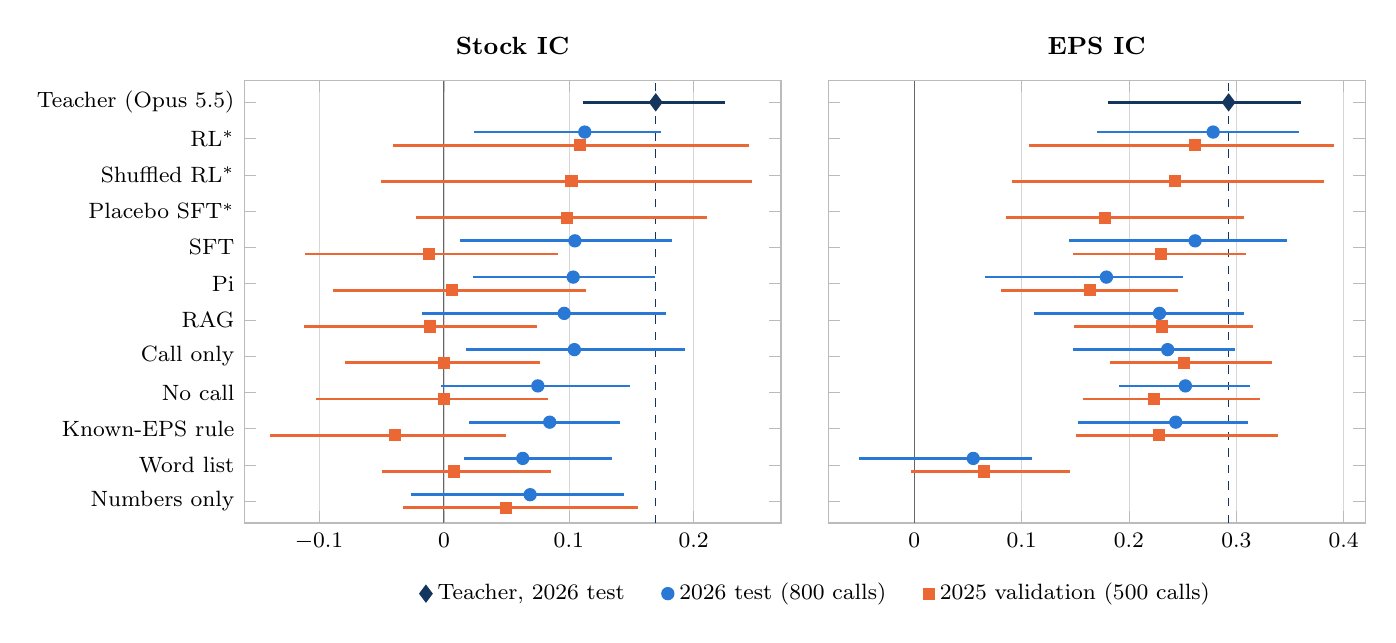
\begin{tikzpicture}
\pgfplotsset{
  panel/.style={
    width=8.4cm, height=7.2cm,
    xmajorgrids, grid style={draw=Rule!60, very thin},
    ymin=0.4, ymax=12.6, ytick={1,...,12},
    tick label style={font=\footnotesize}, label style={font=\footnotesize},
    title style={font=\small\bfseries},
    axis line style={draw=Rule}, tick style={draw=Rule},
    clip=false},
  testpts/.style={only marks, mark=*, mark size=2.2pt, color=TestBlue,
    error bars/.cd, x dir=both, x explicit, error bar style={line width=1pt, color=TestBlue}, error mark=none},
  valpts/.style={only marks, mark=square*, mark size=2pt, color=ValOrange,
    error bars/.cd, x dir=both, x explicit, error bar style={line width=1pt, color=ValOrange}, error mark=none},
  teachpts/.style={only marks, mark=diamond*, mark size=3pt, color=Teacher,
    error bars/.cd, x dir=both, x explicit, error bar style={line width=1pt, color=Teacher}, error mark=none},
}
\begin{groupplot}[group style={group size=2 by 1, horizontal sep=6mm, y descriptions at=edge left},
  panel,
  yticklabels={Numbers only, Word list, Known-EPS rule, No call, Call only, RAG, Pi, SFT, Placebo SFT$^{*}$, Shuffled RL$^{*}$, RL$^{*}$, Teacher (Opus 5.5)}]
%---------------- Stock IC
\nextgroupplot[title={Stock IC}, xmin=-0.16, xmax=0.27, xtick={-0.1,0,0.1,0.2}]
\draw[Muted, thin] (axis cs:0,0.4) -- (axis cs:0,12.6);
\draw[Teacher, dashed, thin] (axis cs:0.16967,0.4) -- (axis cs:0.16967,12.6);
\addplot[teachpts] table[x=x, y=y, x error plus expr=\thisrow{hi}-\thisrow{x}, x error minus expr=\thisrow{x}-\thisrow{lo}] {
x y lo hi
0.16967 12 0.111566 0.225188
};
\addplot[testpts] table[x=x, y expr=\thisrow{y}+0.18, x error plus expr=\thisrow{hi}-\thisrow{x}, x error minus expr=\thisrow{x}-\thisrow{lo}] {
x y lo hi
0.112829 11 0.024371 0.173821
0.104887 8 0.012485 0.182554
0.103539 7 0.0235 0.169278
0.096341 6 -0.01742 0.177762
0.104484 5 0.017609 0.193073
0.075235 4 -0.002426 0.148998
0.084725 3 0.020046 0.140825
0.063137 2 0.016323 0.134258
0.069053 1 -0.026306 0.144315
};
\addplot[valpts] table[x=x, y expr=\thisrow{y}-0.18, x error plus expr=\thisrow{hi}-\thisrow{x}, x error minus expr=\thisrow{x}-\thisrow{lo}] {
x y lo hi
0.108791 11 -0.041079 0.244212
0.102183 10 -0.050373 0.247129
0.098643 9 -0.022741 0.210985
-0.011685 8 -0.111662 0.091508
0.006594 7 -0.088749 0.113591
-0.011199 6 -0.112451 0.074824
-0.000064 5 -0.079122 0.077164
0.000001 4 -0.102648 0.082991
-0.039513 3 -0.139027 0.049976
0.008356 2 -0.049529 0.08577
0.049815 1 -0.033162 0.15567
};
%---------------- EPS IC
\nextgroupplot[title={EPS IC}, xmin=-0.08, xmax=0.42, xtick={0,0.1,0.2,0.3,0.4},
  legend style={font=\footnotesize, at={(-0.02,-0.11)}, anchor=north, draw=none, legend columns=3, /tikz/every even column/.append style={column sep=4mm}}, legend cell align=left]
\draw[Muted, thin] (axis cs:0,0.4) -- (axis cs:0,12.6);
\draw[Teacher, dashed, thin] (axis cs:0.292849,0.4) -- (axis cs:0.292849,12.6);
\addplot[teachpts] table[x=x, y=y, x error plus expr=\thisrow{hi}-\thisrow{x}, x error minus expr=\thisrow{x}-\thisrow{lo}] {
x y lo hi
0.292849 12 0.180774 0.360177
};
\addlegendentry{Teacher, 2026 test}
\addplot[testpts] table[x=x, y expr=\thisrow{y}+0.18, x error plus expr=\thisrow{hi}-\thisrow{x}, x error minus expr=\thisrow{x}-\thisrow{lo}] {
x y lo hi
0.278445 11 0.170475 0.358453
0.261617 8 0.144497 0.34703
0.179057 7 0.065841 0.250109
0.228455 6 0.111383 0.306719
0.236075 5 0.148025 0.299051
0.252586 4 0.190629 0.313115
0.243605 3 0.152325 0.310441
0.055021 2 -0.051498 0.110041
};
\addlegendentry{2026 test (800 calls)}
\addplot[valpts] table[x=x, y expr=\thisrow{y}-0.18, x error plus expr=\thisrow{hi}-\thisrow{x}, x error minus expr=\thisrow{x}-\thisrow{lo}] {
x y lo hi
0.261301 11 0.107405 0.391101
0.242696 10 0.0914 0.381839
0.177528 9 0.085803 0.307281
0.229949 8 0.148268 0.308972
0.163788 7 0.08092 0.245993
0.231128 6 0.148513 0.315765
0.251153 5 0.182054 0.332921
0.223039 4 0.157148 0.322267
0.227773 3 0.150905 0.338829
0.064762 2 -0.003238 0.145014
};
\addlegendentry{2025 validation (500 calls)}
\end{groupplot}
\end{tikzpicture}
\caption{Each setup in two periods, with 95\% week-block ranges. Left: the Stock IC of about 0.10 in 2026 (blue) falls to about zero in 2025 (orange). Right: the EPS forecast holds in both periods, but the facts-only setups (No call, Known-EPS rule) come close. $^{*}$RL and its controls read 300 of the 2025 calls, and these calls were easier for every trained model. The dashed line marks the teacher.}
\label{fig:twoperiods}
\end{figure*}

\textbf{The EPS forecast holds.}
Every setup forecasts the direction of the next EPS change in both periods, with every range above zero.
But most of this signal comes from the facts line.
The call text did not add a clear gain: Call only minus No call was $-0.017$ in 2026 and $+0.028$ in 2025, and both ranges include zero.

\textbf{Stock ranking does not repeat.}
In 2026, four of the five reading setups had a Stock IC with a range above zero.
The top third of calls by $p(\text{BUY})$ beat the bottom third by 4\% to 6\% over 60 sessions.
In 2025, the same setups had Stock ICs from $-0.012$ to $+0.007$.
RL scored 0.109 on its 300 validation calls, but the placebo and the shuffled control scored 0.099 and 0.102 on the same calls.
So those calls were easier, and RL's score is not evidence that its ranking repeats.

\textbf{RL's return does not repeat.}
RL had the highest return after costs among the student setups, $+1.06\%$.
Most of it came from one month: its 51 BUY calls in April 2026 earned $+7.25\%$.
In March and May, its BUY calls lost money after costs.
On the 2025 calls, the same model returned $-2.08\%$.
RL also earned $0.56\%$ more than SFT in 2026, with a range just above zero.
It did so by dropping 49 of SFT's BUY calls, which did 3.5\% worse than their sectors on average.
In 2025, the difference was $-0.15\%$.

\textbf{A lead: the model complements the rules.}
RL's ranks within each month correlate only 0.37 with the Known-EPS rule and 0.24 with the Word list.
The mean of the three ranks had a higher Stock IC than the mean of the two rule ranks: $+0.025$ in 2026 and $+0.026$ in 2025.
The gain has the same size in both periods, but both ranges include zero.

\begin{table*}[t]
\caption{Each signal in two periods. Values in brackets are 95\% week-block ranges of paired differences on the same calls. We chose these checks after we saw the 2026 results. The teacher row uses the 300 check calls (2023 to 2024) as its second period. Status: \emph{Holds}, clear in every period tested, with ranges above zero. \emph{Lead}, about the same gain in both periods, but the ranges include zero. \emph{Not distinguishable}, small values with ranges that include zero. \emph{Did not repeat}, positive in 2026 but zero or negative in 2025. \emph{No gain}, zero or negative in 2026.}
\label{tab:signals}
\footnotesize
\begin{tabularx}{\textwidth}{>{\raggedright\arraybackslash}p{4.4cm} >{\raggedright\arraybackslash}X >{\raggedright\arraybackslash}X >{\raggedright\arraybackslash}p{2.9cm}}
\toprule
Signal & 2026 test & 2025 validation & Status \\
\midrule
Every setup forecasts the EPS direction & EPS IC 0.179 to 0.278, all ranges $>0$ & EPS IC 0.164 to 0.261, all ranges $>0$ & \hold, mostly from the facts line \\
The action follows the read lines & -- & $p(\text{BUY})$ 0.31 $\to$ 0.54 when Demand flips, 200 of 200 calls (Section~\ref{sec:weak}) & \hold \\
The teacher ranks better than RL (Stock IC) & $+0.057$ \rng{0.007}{0.111} \newline Jul--Aug $+0.026$ \rng{$-$0.037}{0.211} & Check calls: $+0.121$ \rng{0.017}{0.259} & \hold, except after the teacher's date \\
The teacher's BUYs earn more than RL's & $+1.06\%$ \rng{0.27}{2.19} \newline Jul--Aug $+0.80\%$ \rng{0.07}{1.46} & -- & \hold \ in 2026 \\
\midrule
RL + two rules beats the two rules (Stock IC) & $+0.025$ \rng{$-$0.016}{0.056} & $+0.026$ \rng{$-$0.036}{0.097} & Lead \\
\midrule
The reading setups rank stocks (Stock IC) & 0.096 to 0.113, 4 of 5 ranges $>0$ & $-$0.012 to 0.007 & Did not repeat \\
Call text adds to the facts line (EPS IC) & $-0.017$ \rng{$-$0.074}{0.014} & $+0.028$ \rng{$-$0.060}{0.089} & No gain \\
RAG beats Call only (Stock IC) & $-0.008$ \rng{$-$0.096}{0.069} & $-0.011$ \rng{$-$0.081}{0.034} & No gain \\
SFT beats RAG (EPS IC) & $+0.033$ \rng{$-$0.004}{0.076} & $-0.001$ \rng{$-$0.044}{0.037} & Did not repeat \\
RL beats SFT (Stock IC) & $+0.008$ \rng{$-$0.023}{0.028} & $+0.018$ \rng{$-$0.042}{0.051} & Not distinguishable \\
RL beats SFT (return after costs) & $+0.56\%$ \rng{0.04}{1.15} & $-0.15\%$ \rng{$-$1.30}{0.87} & Did not repeat \\
RL earns money after costs & $+1.06\%$ \rng{$-$2.28}{3.93} & $-2.08\%$ \rng{$-$6.29}{1.80} & Did not repeat \\
RL beats Shuffled RL (Stock IC) & -- & $+0.007$ \rng{$-$0.039}{0.042} & Not distinguishable \\
\bottomrule
\end{tabularx}
\end{table*}

\subsection{The teacher on the same calls}\label{sec:teacher}

We gave the teacher the 800 test calls with the same prompt and knowledge block as RAG.
On all 800 calls, the teacher ranked stocks better than Pi, SFT, RL and the three rules.
Against RL, the Stock IC gap was $+0.057$ \rng{0.007}{0.111}.
Its BUY calls earned $+1.06\%$ more than RL's \rng{0.27}{2.19}.
On the EPS forecast, the trained students came close: the gap was $+0.031$ for SFT and $+0.014$ for RL, and both ranges include zero.

The teacher's knowledge date is about June 2026.
Thus it can know outcomes of some March to May calls.
The 224 calls from July and August come after that date.
On these calls, the Stock IC gaps are not distinguishable, but the return gaps over SFT and RL stay above zero.
The teacher's own Stock IC stayed about the same (0.170 overall, 0.165 in July and August).
But every student setup and rule had a higher Stock IC in July and August.
Call only (0.192) and No call (0.181) scored above the teacher there.
These two months cover only 5 weeks of calls, so their ranges are wide.
We cannot tell whether the teacher's lead on all 800 calls comes from reading or from memory.

\subsection{Where the student is weak}\label{sec:weak}

\textbf{The action follows the read.}
On 200 validation calls, we forced the Demand line to ``down'' and then to ``up''.
The SFT model's mean $p(\text{BUY})$ rose from 0.31 to 0.54, and it rose on all 200 calls.
After RL, the mean rise was 0.21, on 199 of 200 calls.

\textbf{The read is the weak part.}
On the 300 check calls, the teacher had a Stock IC of 0.151.
The student setups had 0.056 or less (Call only 0.056, RAG $-0.001$, SFT $-0.003$, RL 0.031).
Together with the result above, this locates the gap in the read lines, not in the step from read to action.

\textbf{The student's own searches hurt.}
Pi had a lower EPS IC than RAG (0.179 against 0.228).
When we gave the same tool loop RAG's documents, its EPS IC on 200 shared validation calls rose from 0.14 to 0.22.
RAG had 0.28 on these calls.
So the documents that the small model chose caused most of the loss.

%======================================================================
\section{Discussion and limitations}
%======================================================================

\textbf{One period overstates skill.}
On the 2026 calls alone, our results would support several claims.
The reading setups rank stocks, RL improves on SFT, and RL earns money after costs.
None of these claims survived the 2025 check.
Studies of LLM trading that report one test window~\cite{xiao2024tradingagents,chen2025stockbench} can carry the same risk.
We suggest a second period and a shuffled-label control as minimum checks.

\textbf{The signal that holds is mostly known numbers.}
The EPS forecast is the one result that holds, but the Known-EPS rule reproduces most of it.
Quarterly EPS changes are autocorrelated, and prices drift after earnings surprises~\cite{bernardthomas1990}.
A useful model must add to this rule, and our lead suggests where to look.

\textbf{Limitations.}
The test set has 800 calls in 22 weeks.
``Not distinguishable'' means that this test cannot detect a difference.
It does not prove that the difference is zero.
We tested one student model, one horizon of 60 sessions and one group of small companies.
We chose the second-period checks after we saw the 2026 results.
The 2025 calls may be inside the student's pretraining data, and masking does not hide every company.
The training calls (2021 to 2024) are older still, and SFT or RL on them can reward memory~\cite{koijenlevy2026}.
The trained models give very small probabilities to the allowed answer words in free text.
The scores compare the allowed values with each other, so they stay valid.
But the trained models would not follow the seven-line format without constrained reading.

%======================================================================
\section{Future work}\label{sec:future}
%======================================================================

\textbf{A confirmatory test.}
The sealed test set has calls from the same months as the test set.
Before we open it, we will write down the checks, their pass rules and an estimate of the test's power.
The power is the chance to detect a real gain.
Then we will open the set once.
The first check is the lead: whether RL plus the rules beats the rules alone.

\textbf{Larger RL on a smaller model.}
The RL step used only 400 calls and 100 updates.
Many more calls from 2016 to 2024 have both text and outcomes.
A model of the same family with 2 billion parameters runs faster and recalls company identities less often than Qwen3.5-9B in our tests.
We plan one large RL run of 10{,}000 calls with checkpoints.
A learning curve on held-out 2025 calls and a shuffled-reward control of the same size will test it.

\textbf{Rewards that pay only for what the call adds.}
An EPS reward can pay only for the part of the EPS change that the Known-EPS rule does not forecast.
A trade reward on the within-month rank matches the Stock IC and resists outliers.

\textbf{Teacher reads with a student action.}
If the student's Stock IC moves toward the teacher's when it gets the teacher's read lines, then the read lines are the part to train.

\textbf{Robustness.}
Further work should add more training seeds, a second model family, and returns adjusted for market, size and momentum factors.
A memorization test with anonymized calls before and after the teacher's knowledge date can separate reading from memory~\cite{glassermanlin2023}.

%======================================================================
\section{Reproducibility}
%======================================================================

All runs used one Apple M3 Pro laptop with 18\,GB of memory and MLX.\footnote{\url{https://github.com/ml-explore/mlx}}
An SFT run took about 8 hours, an RL run about 6 hours, and one setup's read of 800 calls about 3 hours.
The repository holds the code, the adapters, every model answer, the test outcomes, and the scripts that rebuild every table.\footnote{\url{https://github.com/nityarai08/earnings-call-distillation}}
One script recomputes the main table from the released files in about one minute.
We do not redistribute transcript text.
The sealed test outcomes stay closed.

\bibliographystyle{ACM-Reference-Format}
\bibliography{refs}

\end{document}
